\lab{Algorithms}{Complex Numbers}{Complex Numbers}

\objective{Learn to perform basic computation and visualization with complex numbers.}

\section*{Arithmetic with complex numbers}
Computationally, complex numbers are really just a pair of floating point numbers.
The first is understood to represent the real part of the complex number.
The second is understood to represent the imaginary part.
In Python, a complex number $a + b i$ can be defined using either of the following methods
\begin{lstlisting}
complex(a, b)
a + 1.0j * b
\end{lstlisting}
Python lets us define purely imaginary numbers using the syntax shown there with \li{j}.
As another example, $2 i$ would be \li{2.0j}.

Python also includes the built in \li{cmath} library.
This library provides basic math functions for complex numbers.
For examle, the functions \li{polar} and \li{rect} can be used to convert to and from polar coordinates (discussed below).
It also includes basic functions like \li{sin}, \li{cos}, etc. with their domains extended to the complex numbers.

There are some computational advantages and disadvantages to using complex numbers.
Addition or subtraction between two complex numbers now requires two floating point operations (one for each part of the number), so it takes longer.
Multiplicatoin and division are more costly.
Mutliplication is easily seen to take 4 floating point multiplies and two floating point adds instead of just a single floating point multiply.
The fact that there two numbers are stored also increases the amount of floating point error that can be created in each computation.

Most of the basic functions in NumPy support complex numbers.
Fore example, \li{numpy.absolute} will take the absolute value of a complex number without any trouble.
You can also acces the real and imaginary parts of a complex array via the \li{real} and \li{imag} attributes.
For example,
\begin{lstlisting}
import numpy as np
from numpy.random import rand
Z = rand(10) + 1.0j * rand(10)
# print real part
print Z.real
# print imaginary part
print Z.imag
\end{lstlisting}

The complex conjugate of a complex number or array can be obtained using the \li{conjugate} method.
For example, if \li{A} is a complex number or complex array, its conjugate (or elementwise conjugate) is obtained via
\begin{lstlisting}
A.conjugate()
\end{lstlisting}

\section*{Polar Representation of Complex Numbers}

One of the most important results in Complex Analysis is Euler's Formula.
It states that:

$$e^{i\theta}=cos(\theta)+i sin(\theta)$$.

One way to derive this important result is to consider the taylor series expansion of each of the functions involved.

From this formula, we can see that $e^x$ maps the imaginary axis onto the unit circle on the complex plane.
From our knowledge of the sine and cosine functios, we can also know that this mapping has a period of $2\pi$.
From here, notice that we may represent any number on the complex plane in the form $r e^{i\theta}$ for $r\geq 0$ and $0 \leq \theta \leq 2\pi$.
This is what is known as the polar representation of a complex number.
Conceptually, it is \emph{identical} to the polar representation of points in the standard cartesian plane.
The primary difference is that, here we define a map from $\mathbb{C}$ to the polar coordinates instead of from $\mathbb{R^2}$ to the polar coordinates.
The number $\theta$ is known as the argument, or phase, of a complex number.
The number $r$ is known as the modulus, magnitude, or absolute value of a complex number.
In the complex plane we define $|z|$ as the modulus of $z$ and $arg(z)$ as the argument of $z$.

\section*{Multi-Valued Functions}

Another important topic in Complex Analysis is the study of multiple valued functions.
These functions arise as we consider the inverses of functions that are not strictly one to one on the complex plane.
A classic example is $\sqrt{x}$, which may take two values for every nonzero point of the complex plane.

In the Real numbers we worked with functions like this by simply restricting their output on a certain domain.
We can do a similar thing in the Complex plane.
Loosely speaking, such a restriction is called a branch.
Computationally we restrict the output to a single portion of the actual possible values of the multifunction.
We call inverse functions that have multiple values like this ``multi-valued functions" or ``multifuctions."
We can still visualize the ``Riemann surfaces" of such multi-valued functions in the complex plane.
Figure \ref{fig:sqrt_riemann_surface} shows the Riemann surfaces for $\sqrt{z}$ in the complex plane.
Riemann surfaces are simple examples of manifolds.

\begin{figure}
\begin{subfigure}{.49\textwidth}
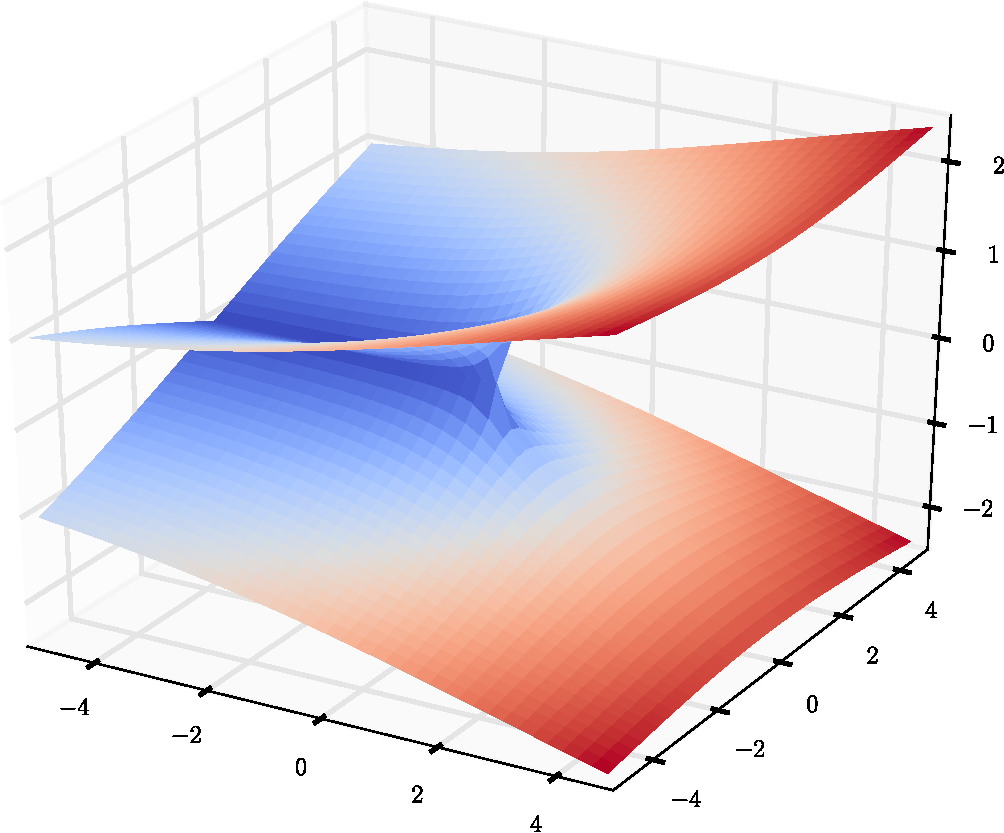
\includegraphics[width=\textwidth]{sqrt_riemann_surface_1}
\end{subfigure}
\begin{subfigure}{.49\textwidth}
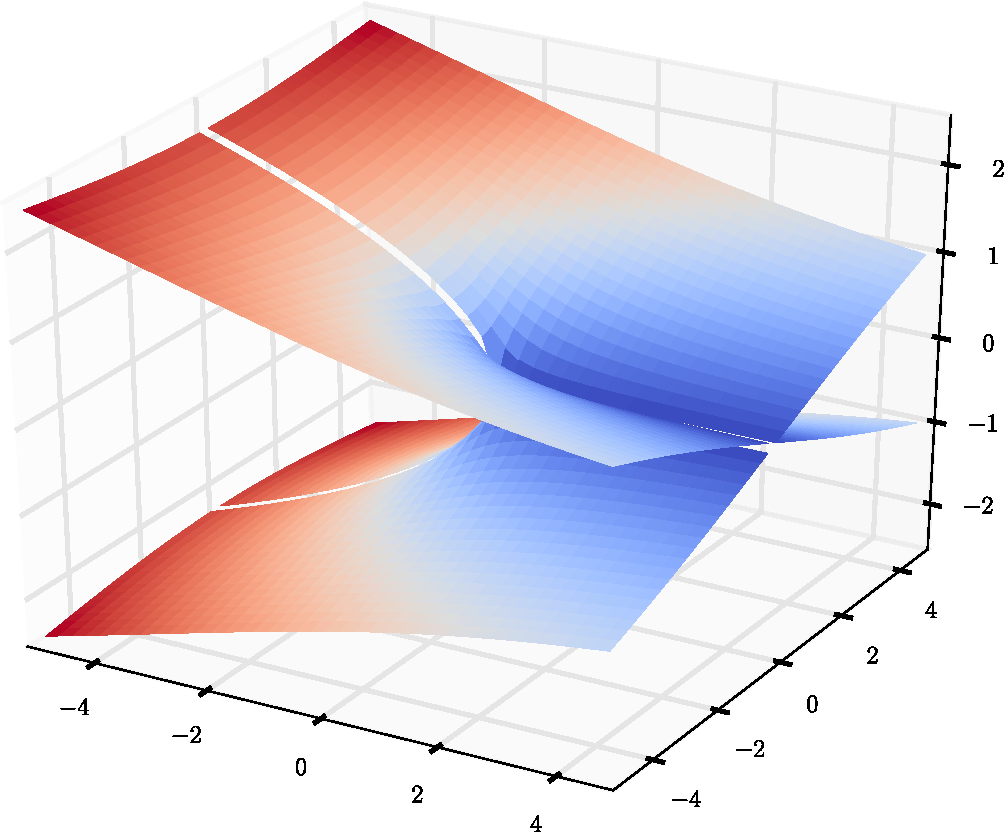
\includegraphics[width=\textwidth]{sqrt_riemann_surface_2}
\end{subfigure}
\caption{The real and imaginary parts of the function $\sqrt{z}$.}
\label{fig:sqrt_riemann_surface}
\end{figure}

These are some very basic examples.
Riemann surfaces can be very complex.
Another simple example is $\ln\left(z\right)$ which has a single value for the real part and infinitely many possible values for its imaginary part.
The Riemann surface for the imaginary part of $\ln\left(z\right)$ is shown in Figure \ref{fig:log_riemann_surface}.
Note that Figure \ref{fig:log_riemann_surface} is only a portion of the Riemann surface of the imaginary part of $\ln\left(z\right)$.
The full surface is, in actuality, an infinite spiral that repeats every $2\pi$.
This is because for any complex $z\neq 0$, we have $e^z=e^{z+2n\pi}$ where $n$ is any integer.

\begin{figure}
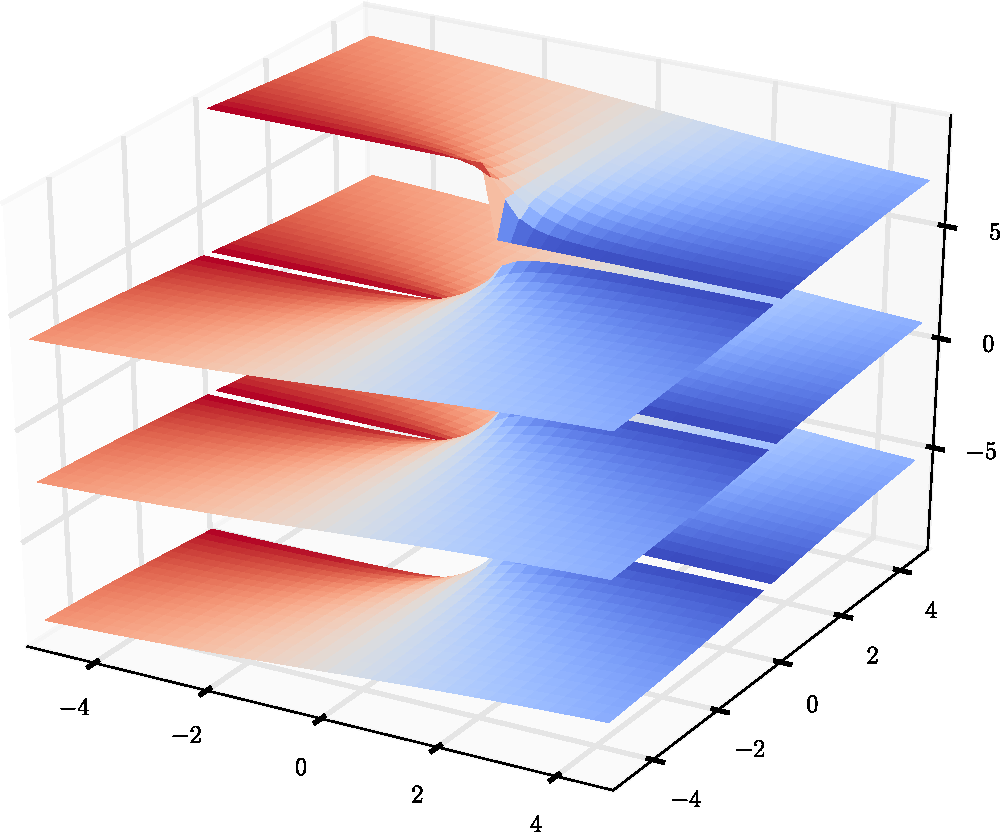
\includegraphics[width=\textwidth]{log_riemann_surface}
\caption{Riemann surface plot of a portion of the imaginary part of $\ln\left(z\right)$}
\label{fig:log_riemann_surface}
\end{figure}

Figure \ref{fig:arctan_riemann_surface} shows the real part of the riemann surface of $\arctan\left(z\right)$
All three of the functions we have plotted can be made analytic at almost any point, except at their singularities, but that depends on how we cut the domain to give it a single value.
When Integrating such functions, be careful about integrating across such cuts in the domain.

\begin{figure}
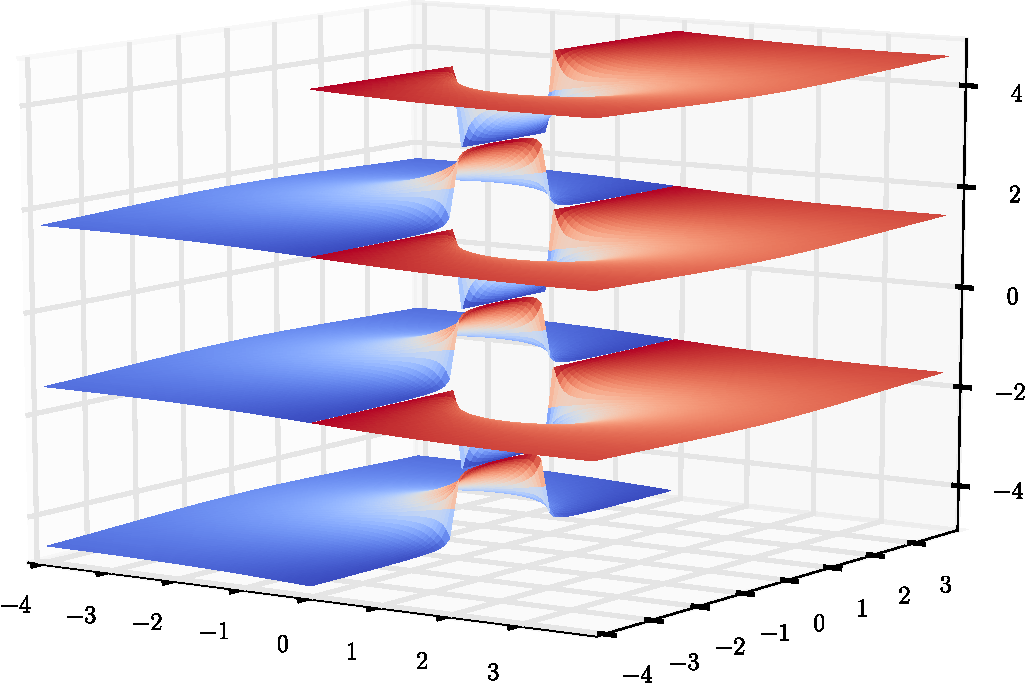
\includegraphics[width=\textwidth]{arctan_riemann_surface}
\caption{Even the Riemann surface of $\arctan(z)$ becomes increasingly complex.
This is a graph of a portion of the Riemann surface for the real part of $\arctan(z)$.}
\label{fig:arctan_riemann_surface}
\end{figure}

\begin{problem}
Write two functions, both accepting accept a natural number $n$.
Have one function plot the riemann surface for the real part $\sqrt[n]{z}$ and the other plot the imaginary part.

Hint: use the polar form of complex numbers to obtain the different solutions at each point.
You can plot several separate surfaces that agree on their boundaries.
The surfaces you will want to plot will be the surfaces of the form
\[\sqrt[n]{r} e^{i \frac{\theta + 2 \pi k}{n}}\]
where $r e^{i \theta}$ is the polar form of the complex number and $k = 0, 1, \dots, n-1$.
\end{problem}